\documentclass[conference]{IEEEtran}
\IEEEoverridecommandlockouts
% The preceding line is only needed to identify funding in the first footnote. If that is unneeded, please comment it out.
\usepackage{cite}
\usepackage{amsmath,amssymb,amsfonts}
\usepackage{algorithmic}
\usepackage{graphicx}
\usepackage{textcomp}
\usepackage{xcolor}
\usepackage{tikz}
\usepackage{tikz-qtree}
\usetikzlibrary{shapes,trees,fit,decorations.pathreplacing,arrows.meta}
\usepackage{color,soul}

\def\BibTeX{{\rm B\kern-.05em{\sc i\kern-.025em b}\kern-.08em
    T\kern-.1667em\lower.7ex\hbox{E}\kern-.125emX}}
\begin{document}

\title{Geo-referenced Photo Management System\\
%{\footnotesize \textsuperscript{*}Relation for the Context Aware System course project}
}

\author{\IEEEauthorblockN{Gabriele Spina}
\IEEEauthorblockA{\textit{University of Bologna} \\
\textit{Second Cycle Degree in Computer Science}\\
Bologna, Italy\\
gabriele.spina2@studio.unibo.it}
}

\maketitle

\begin{abstract}
This document illustrates the deployment phases of a geo-referenced photo management system, made for the final project of the Context Aware Systems course at University of Bologna.
\end{abstract}

\section{Introduction}
The geo-localization of the photos is a functional information. Using that information during the process of design and implementation of a photo management system can lead the user to take benefit from a great number of interesting features. 
The aim is to implement a Mobile Application where photos can be visualized, taken, etc., that interacts with a database that contains the information about the photos as the localization. Moreover, a Web Dashboard to visualize the photos on the map and other features related to spatial processing.
A user will take photos with the mobile application while traveling or during his normal day, then he will interact with the dashboard to retrieve his movements during the trip or the day, or even he will be able to recover old photos in a fastest way if knows the location.

\section{Design}
\subsection{Database}
The geographic database is composed by two tables, one for the photos, in Table~\ref{table:mf}, and one for the collections in which they reside, in Table~\ref{table:col}.

\begin{table}[h!]
\centering
\begin{tabular}{llll}
\multicolumn{4}{c}{Media Files}                                            \\ \hline
\multicolumn{2}{l|}{id}             & \multicolumn{2}{l}{serial}           \\
\multicolumn{2}{l|}{name}           & \multicolumn{2}{l}{varchar}          \\
\multicolumn{2}{l|}{date}           & \multicolumn{2}{l}{timestamp}        \\
\multicolumn{2}{l|}{image}          & \multicolumn{2}{l}{bytea}            \\
\multicolumn{2}{l|}{position}       & \multicolumn{2}{l}{geography(point)} \\
\multicolumn{2}{l|}{collection\_id} & \multicolumn{2}{l}{int}             
\end{tabular}
\caption{Media files table design.}
\label{table:mf}
\end{table}

\begin{table}[h!]
\centering
\begin{tabular}{llll}
\multicolumn{4}{c}{Collections}                                     \\ \hline
\multicolumn{2}{l|}{collection\_id} & \multicolumn{2}{l}{serial}    \\
\multicolumn{2}{l|}{name}           & \multicolumn{2}{l}{varchar}   \\
\multicolumn{2}{l|}{created\_at}    & \multicolumn{2}{l}{timestamp}
\end{tabular}
\caption{Collections table design.}
\label{table:col}
\end{table}

For each media file we store the raw data into an array of bytes, the position as a coordinates point, the referring collection\_id where the image resides, and other information.
For the collections we store the name, the date of creation and a unique identifier.    

\subsection{Mobile Application}
The mobile application is structured by an home screen with the list of the collections, with an image as preview for each one. Then there is the location, a button to open the camera and take new photos, a button to create a new collection, and a button to retrieve the photos taken nearest to the current position. 

\medskip

By clicking on a collection another screen is opened with the list of all the photos of the collection with the possibility to visualize a single photo in a another screen and delete it if necessary.

\medskip

By clicking the add collection button a pop-up window is opened asking the name for the new collection, after the input the camera screen is opened to take the first photo of the collection.

\medskip

The camera screen got the camera visualization and the button to acquire the photo. By clicking the button another screen is opened where is asked the name for the photo and the collection to which add it.

\medskip

The last part is when the button to retrieve the photos taken nearest to the current position is pressed. A pop-up window is opened that asks the number of photo to retrieve. Then a screen is opened with the list of the nearest photos, similar to the one of the collection screen. 

\subsection{Dashboard Web}
The dashboard is composed of two web pages, a home page with the map and a secondary page to visualize the photos like a gallery. 

\medskip

The homepage displays the map on half of the screen and on the other half there are the controls to interact with the map. Specifically there are three categories of controls: \begin{itemize}
\item \textbf{Add images}: the user can upload a single image or a folder specifying the collection where to add the photos and the position. For the folder case as all the photos will be saved with the same position, there is the possibility to save the photos with a perturbed position at a maximum given distance range.   
\item \textbf{Add GeoJson files}: the user can upload a geojson file containing zones to visualize them on the map. Then a zone can be clicked to visualize only the photos taken in that specific place. Moreover, the zones can be colored on the base of the amount of photo taken in each one. 
\item \textbf{Filter the markers of photos on the map}: the markers representing the photos on the map can be divided in groups and visualized with different colors. There is the possibility to find the places where more photos were taken by visualizing a heatmap. Then there is the possibility to build a path between all the photos of a collection in chronological order to reconstruct the crossed trail taking photos.    
\end{itemize}

\section{Implementation}
\subsection{Database}
The backend is a \textit{PostreSQL} database that support spatial queries. The tables "collections" and "media\_files" are constructed as described in previous section. Then the database has been partially populated with some photos, then photos will be added via mobile app or dashboard web. As photos in high resolution will result in too much long byte arrays, all photos are compressed before being added to the database and decompressed after extracted. 

\subsection{Mobile Application}
The mobile application is implemented with \textit{Python} programming language and the \textit{Kivy} library. Kivy has been chosen since it is cross-platform so the application can be deployed on Windows, Linux, macOS, iOS and Android. The application interacts with the database to fetch the informations about collections and photos, and to modify those informations. 

\subsection{Dashboard Web}
The dashboard is implemented using \textit{HTML}, \textit{JavaScript}, and \textit{Leaflet} library. To interact with the database as backend language is used \textit{Python} with \textit{Flask} library. The choose of Flask is due to its minimalist approach that consent to build the applications from scratch, granting great flexibility.

\section{Results}
The system constructed works really well in a local environment with a small amount of data. In Figure~\ref{fig:dash} there is the screenshot of the home page the web dashboard. In Figure~\ref{fig:app} there is the screenshot of the home screen of the mobile application. 

\medskip   

The scalability of the system with a greater amount of data is not so good, mainly because the photos are stored directly as byte arrays in the database. 

\begin{figure}[h!]
\centering
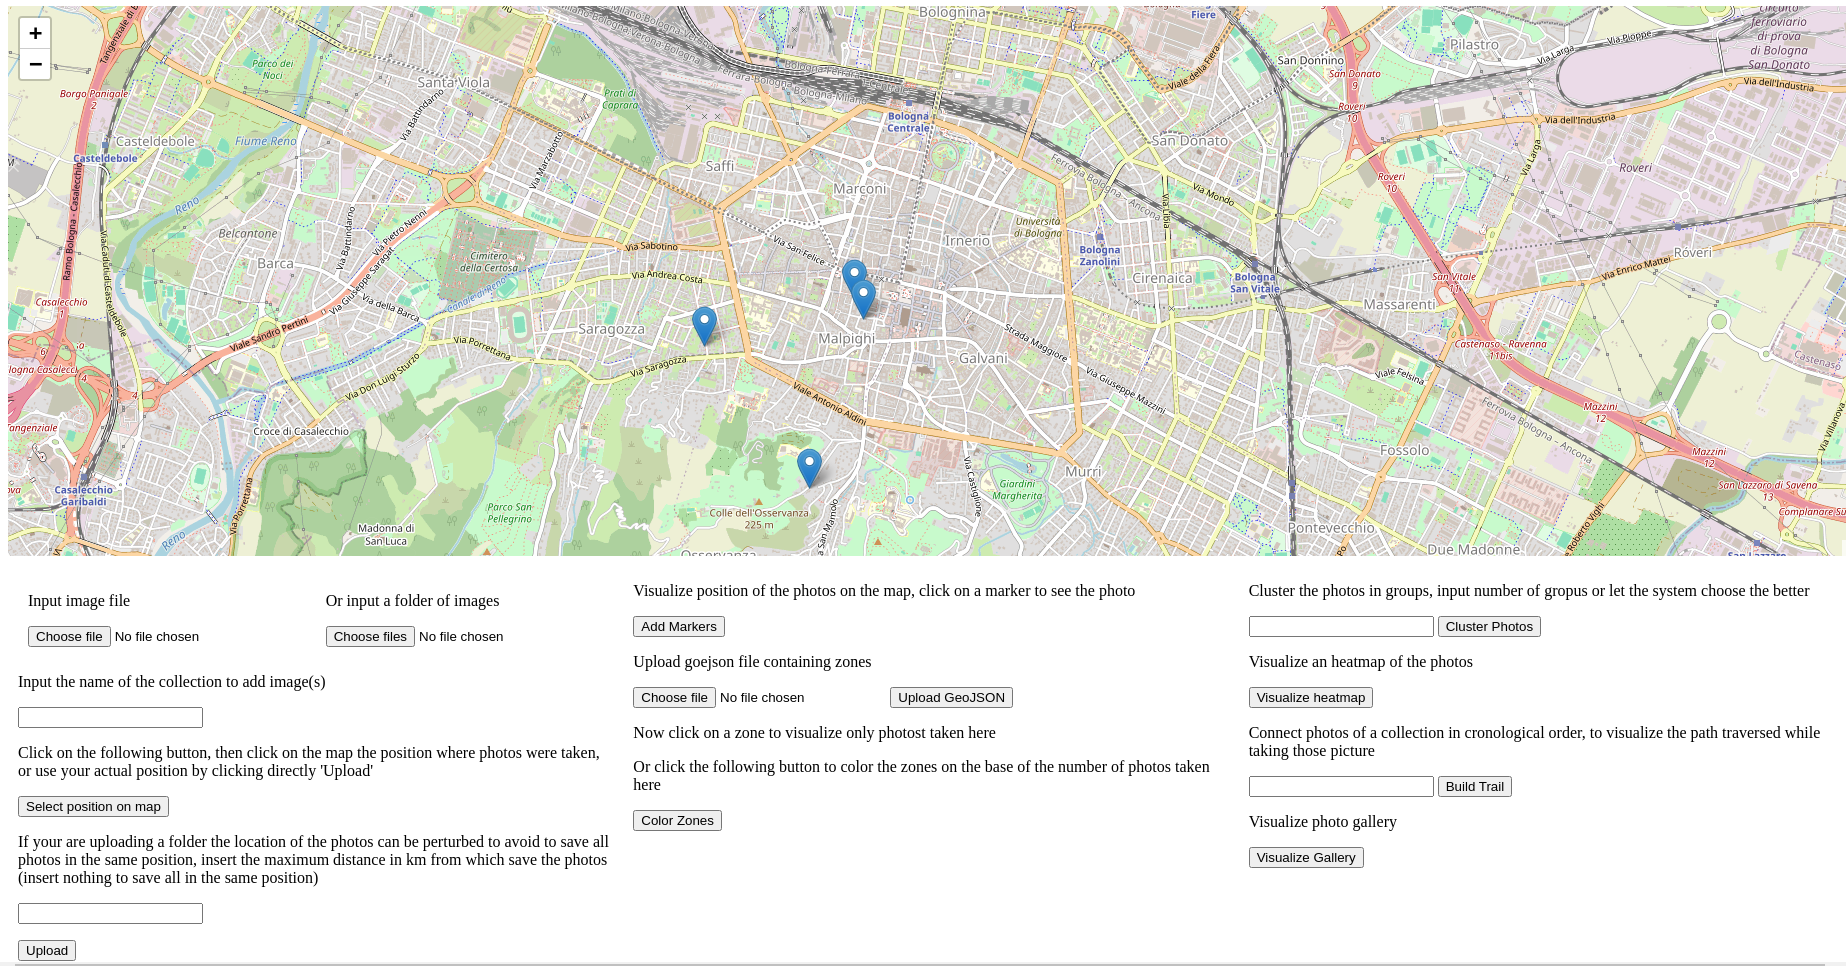
\includegraphics[width=.5\textwidth]{dash.png}
\caption{Web dashboard main screen}
\label{fig:dash}
\end{figure}

\begin{figure}[h!]
\centering
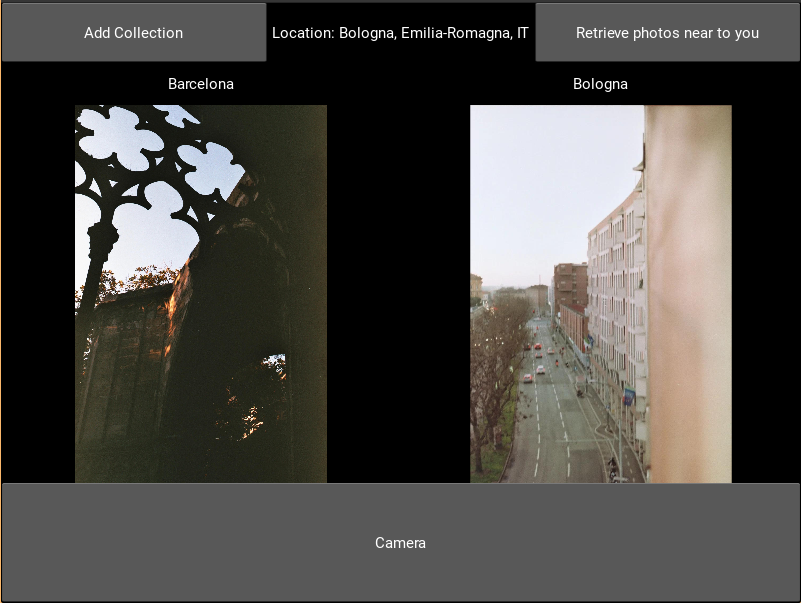
\includegraphics[width=.4\textwidth]{app.png}
\caption{Mobile application main screen}
\label{fig:app}
\end{figure}


\end{document}
